\section{Marco Teórico}

\subsection{Gamma-Ray Bursts}

\subsubsection{Descubrimiento de los GRB}

En 1963, los Estados Unidos lanzaron el satélite VELA, cuyo objetivo era vigilar que no se realizaran pruebas de bombas nucleares. Una explosión nuclear emite una gran cantidad de rayos X, rayos Gamma y neutrones, por lo que Vela tenía instrumentos para la detección de estos residuos \cite{Rosswog2009}. En 1967, el satélite Vela 4 detectó un destello de rayos gamma que no coincidía con lo esperado de una explosión nuclear. En lugar de eso, este pulso tenía una estructura distinta y una duración de varios segundos. 

Los datos de esa detección permanecieron clasificados y sin mayor relevancia hasta que varios años después un equipo de científicos en el \textbf{Laboratorio Nacional de Los Álamos}, liderado por Ray W. Klebesadel concluyeron que este destello y muchos otros procedían de fuentes externas al sistema solar \cite{Klebesadel1973}. 

\subsubsection{¿Qué es un GRB?}
%RECOMENDACIÓN: cAMBIAR EL FORMATO DE PREGUNTA

Los estallidos de rayos gamma (GRBs) son fenómenos altamente energéticos, pues pueden emitir fotones que van desde decenas de keV hasta varios GeV. Estos fenómenos tienen una naturaleza transitoria, pues pueden durar unos cuantos segundos. Además, ocurren a un ritmo de unos cuantos al día en todo el Universo. 

Si supusiéramos que un GRB es una fuente que emite energía de forma isotrópica, este liberaría del orden de $10^{51}-10^{54}$ erg en la banda de la energía gamma en una escala de tiempo que duraría unos cuantos segundos o minutos. Sin embargo, esta no es la forma en la que los GRBs emiten toda esa energía, sino que estos la liberan en forma de un chorro relativista muy colimado, es decir que puede tener ángulos de apertura de entre uno a 10 grados. Si se aplicara esta corrección de geometría, la emisión total disminuye hasta en tres órdenes de magnitud \cite{Meszaros2006}.

Cuando se observa la curva de luz emitida por un GRB, se pueden diferenciar dos fases claras: 

\paragraph{Fase Prompt:}
Esta es la emisión que marca el inicio del estallido y es la que le da nombre al fenómeno, pues corresponde a la radiación gamma observada en segundos. La curva de luz durante esta fase es sumamente errática e impredecible: puede presentar un único pulso suave o una sucesión caótica de picos y valles con variabilidad en escalas de milisegundos \cite{Piran2000}. Esta variabilidad rápida es una de las razones por las que se sabe que la fuente es compacta. La emisión sugiere un mecanismo interno del chorro relativista, como ondas de choque generadas por la interacción de capas de material eyectadas a distintas velocidades (\textit{internal shocks}) o procesos de disipación magnética \cite{Meszaros2006, Zhang2004}.

Espectralmente, la emisión prompt se describe en primera instancia mediante la función de Band, un modelo que está formado por dos leyes de potencia unidas suavemente en una energía de quiebre, esto ayuda a ajustar la porción de baja energía con la de alta energía del espectro observado \cite{Band1993}.

\paragraph{Fase Afterglow:}
Además de la emisión prompt, hay una emisión de menor intensidad que decae de forma suave y progresiva en rayos X, óptico y radio, detectable durante días, semanas o incluso meses después del estallido inicial \cite{MeszarosRees1997}. Esta fase, conocida como \textit{afterglow}, fue predicha teóricamente antes de ser observada, en el marco del modelo de bola de fuego relativista (\textit{fireball model}), el cual propone que el afterglow se origina cuando el chorro relativista inicia su desaceleración por la interacción con el medio circundante (ya sea el medio interestelar o el viento estelar previamente perdido por la estrella progenitora), generando una onda de choque externa que acelera partículas que radian emisión sincrotrón \cite{MeszarosRees1997}.

La confirmación observacional de esta predicción llegó en 1997, cuando el satélite italo-neerlandés \textbf{BeppoSAX} logró localizar con precisión, por primera vez, un afterglow de rayos X asociado al GRB970228 \cite{Costa1997}, seguido poco después por la detección de su contraparte óptica \cite{vanParadijs1997}. Este hallazgo no solo confirmó el modelo de bola de fuego, sino que permitió medir por primera vez el corrimiento al rojo de un GRB, estableciendo de manera definitiva que estas explosiones ocurren a distancias cosmológicas.

\subsubsection{Clasificación de los GRB}

Desde los primeros catálogos sistemáticos de GRBs recopilados por el instrumento BATSE a bordo del \textit{Compton Gamma-Ray Observatory}, se observó que la distribución de duraciones de los estallidos ($T_{90}$, el tiempo durante el cual se acumula entre el 5\% y el 95\% de la fluencia total) no era uniforme, sino que presentaba dos grupos distintivos \cite{Kouveliotou1993}, correlacionados con la dureza espectral de los GRBs: los estallidos cortos tienden a ser más duros (con más fotones de alta energía), mientras que los largos tienden a ser más blandos. A partir de esta observación surgió la clasificación de los GRBs en dos grandes categorías:

\begin{itemize}
    \item \textbf{GRBs largos} ($T_{90} > 2$ s): Se asocian al colapso gravitacional del núcleo de estrellas masivas y de rápida rotación, en un proceso conocido como modelo del \textit{colapsar}. El núcleo colapsa directamente para formar un agujero negro rodeado de un disco de acreción, en lugar de producir una supernova convencional \cite{Woosley1993, MacFadyenWoosley1999}. Esta hipótesis se ha visto reforzada por la asociación observacional recurrente entre GRBs largos y supernovas de tipo Ic de línea ancha, así como por su tendencia a ser localizados en regiones de formación estelar activa dentro de sus galaxias anfitrionas.
    
    \item \textbf{GRBs cortos} ($T_{90} < 2$ s): Se atribuyen a la colisión de sistemas binarios compactos, típicamente dos estrellas de neutrones o una estrella de neutrones y un agujero negro. Esta hipótesis fue propuesta desde 1989 \cite{Eichler1989} y fue confirmada de manera contundente en 2017, con la detección conjunta del evento de ondas gravitacionales GW170817 y el GRB170817A de corta duración.
\end{itemize}


Cabe destacar que esta clasificación basada únicamente en la duración no es estricta, pues existen GRBs que, a pesar de tener una duración corta, presentan características espectrales o entorno más propios de un GRB largo (y viceversa). Por lo que en la literatura reciente se ha propuesto complementar esta división con criterios adicionales relacionados con el progenitor físico \cite{Zhang2006}.



\subsubsection{Espectro de los GRB}

Además de la variabilidad temporal que ya se describió para la fase prompt, la otra propiedad fundamental que caracteriza a un GRB es la forma de su espectro de energía, es decir, cómo se distribuye el número de fotones en función de su energía. Como se mencionó previamente, el espectro de la emisión prompt se describe comúnmente mediante la función de Band, un modelo empírico compuesto por dos leyes de potencia unidas suavemente en una energía de quiebre $E_{peak}$ \cite{Band1993}. Esta función ha demostrado ajustar de manera adecuada el espectro promediado en el tiempo de la mayoría de los GRBs observados en el rango de energía de instrumentos como BATSE y GBM (decenas de keV hasta pocos MeV) \cite{Preece2000}.

Sin embargo, cuando se analiza específicamente la emisión detectada en el rango de energía del LAT (por encima de $\sim$100~MeV), el comportamiento espectral suele simplificarse considerablemente. Esto se debe a que, en la mayoría de los GRBs, la energía de quiebre $E_{peak}$ de la función de Band se encuentra por debajo del umbral de sensibilidad del LAT, de modo que los fotones detectados por este instrumento corresponden casi en su totalidad a la cola de alta energía del espectro, la cual puede aproximarse adecuadamente mediante una \textbf{ley de potencia simple} (\textit{simple power-law}) \cite{Ackermann2013}:

\begin{equation}
    N(E) \ \propto \ E^{-\Gamma}
\end{equation}

donde $N(E)$ es el número de fotones por unidad de energía, unidad de área y unidad de tiempo, y $\Gamma$ es el \textbf{índice fotónico} (\textit{photon index}), que caracteriza la dureza del espectro. Valores de $\Gamma$ cercanos a 2 corresponden a espectros más duros (mayor proporción de fotones de alta energía), mientras que valores de $\Gamma \gtrsim 2$ corresponden a espectros más suaves. Es importante distinguir el índice fotónico $\Gamma$ del índice espectral de energía $\alpha$, definido a partir del flujo de energía $F(E) \propto E^{-\alpha}$, y que se relaciona con el anterior mediante $\alpha = \Gamma - 1$.

Este modelo de ley de potencia simple no es únicamente una simplificación conveniente, sino que tiene un origen físico. Dentro del marco del modelo de bola de fuego relativista, tanto la emisión prompt como la del afterglow se explican mediante radiación sincrotrón (y, en algunos casos, radiación por efecto Compton inverso, en el que los electrones ceden parte de su energía a fotones del entorno) producida por electrones acelerados a energías relativistas en los choques internos y externos del chorro \cite{Meszaros2006, Sari1998}. En el régimen en el que la distribución de energía de estos electrones sigue una ley de potencia ($N(\gamma_e) \propto \gamma_e^{-p}$), la emisión sincrotrón resultante produce naturalmente un espectro de fotones que también sigue una ley de potencia en ciertos rangos de energía, con un índice $\Gamma$ directamente relacionado con el índice $p$ de la distribución de electrones acelerados. Este marco teórico, conocido como las \textit{relaciones de cierre} (\textit{closure relations}) del modelo de bola de fuego, permite conectar el índice espectral medido observacionalmente con las propiedades microfísicas del proceso de aceleración de partículas en el chorro relativista \cite{Sari1998, Zhang2004}.

En la práctica, este es precisamente el modelo utilizado para caracterizar el espectro de alta energía de un GRB observado por el LAT. El objetivo del ajuste es estimar el valor de $\Gamma$ que mejor reproduce los conteos de fotones observados, y a partir de este, inferir propiedades físicas de la emisión de alta energía del estallido.



\subsection{Fermi Large Area Telescope (LAT)}


El LAT es el instrumento principal del telescopio espacial Fermi, diseñado para detectar rayos gamma entre 20~MeV y 300~GeV \cite{Atwood2009}. Su campo de visión es extremadamente amplio, cubre cerca del 20$\%$ del cielo en cualquier instante. En su modo principal de operación, el \textbf{Sky Survey}, el satélite completa una órbita cada $\sim$96~minutos. Realiza un barrido continuo que expone todas las regiones del cielo aproximadamente cada 3~horas, cubriendo la totalidad de la esfera celeste en cuestión de horas a días \cite{Atwood2009}. Esto contrasta con el GBM, que monitorea de forma simultánea prácticamente todo el cielo no ocultado por la Tierra \cite{Meegan2009}.

La detección de rayos gamma no es directa, sino que se infiere a partir del par de partículas cargadas producidas al interactuar con el detector. Internamente, el LAT está compuesto por tres subsistemas principales \cite{Atwood2009}: un \textbf{Tracker} de silicio (TKR), que convierte el fotón incidente en un par electrón-positrón y reconstruye su trayectoria para determinar la dirección de arribo del fotón; un \textbf{Calorímetro} de CsI(Tl) (CAL), que mide la energía total del fotón a partir de la cascada electromagnética producida por dicho par; y un \textbf{Detector de Anticoincidencia} segmentado (ACD), que rodea al instrumento y permite rechazar el abundante fondo de rayos cósmicos cargados. Cada vez que estos subsistemas registran una señal se guarda un \textit{evento}: el conjunto de lecturas del TKR, el CAL y el ACD que, una vez reconstruido, puede corresponder a un fotón o a una partícula cargada. Un sistema electrónico de trigger y filtrado a bordo decide, en tiempo real, qué eventos se transmiten a Tierra, dado el limitado ancho de banda disponible.

La calibración del instrumento queda resumida en las \textbf{funciones de respuesta del instrumento} (\textit{Instrument Response Functions}, IRFs), que describen cómo responde el LAT a un fotón incidente y tienen tres partes: el área efectiva (cuántos cm$^2$ de detector ``ve'' un fotón según su energía y su ángulo de llegada), la PSF (cuánto se dispersa la dirección reconstruida alrededor de la verdadera) y la dispersión en energía (cuánto difiere la energía reconstruida de la real). Cada clase de eventos tiene su propia IRF, porque los cortes de reconstrucción cambian la respuesta; en este trabajo se usan \texttt{P8R3\_TRANSIENT020\_V3} para la fase prompt y \texttt{P8R3\_SOURCE\_V3} para la emisión extendida. Las IRFs aparecen en casi todos los pasos del análisis, pues son lo que permite pasar de conteos detectados a magnitudes físicas.

\begin{figure}[h!]
    \centering
    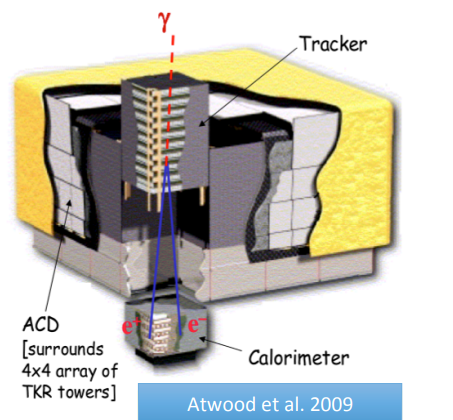
\includegraphics[scale=0.45]{PNGs/Estructura.png}
    \caption{Estructura interna del LAT}
    \label{fig:placeholder}
\end{figure}

\subsection{Fermitools}


Este es el paquete oficial de software desarrollado por el \textit{Fermi Science Support Center} para el análisis de los datos del LAT y el GBM \cite{Fermitools2019}. Se distribuye como un paquete de Python instalable mediante \texttt{conda}, y contiene el conjunto de herramientas de línea de comandos (\texttt{gtselect}, \texttt{gtmktime}, \texttt{gtbin}, \texttt{gtlike}, entre otras) necesarias para procesar los archivos FITS obtenidos del \textit{LAT Photon, Event and Spacecraft Data Query}. Estas funciones nos permiten generar desde la selección espacial, temporal y energética de eventos, hasta el cálculo de la exposición del instrumento y el ajuste de modelos espectrales mediante métodos de máxima verosimilitud. Estas herramientas se apoyan en las IRFs descritas en la sección anterior para convertir los conteos de fotones detectados en magnitudes físicas como flujos, espectros y curvas de luz \cite{FSSCCicerone}. El detalle específico de cada función utilizada se describe en la sección de Metodología.